\section{Data and Methods}
\label{sec:data_methods}

\subsection{Hydrodynamic model}
\label{sec:methods_model}

Circulation was simulated with D-Flow Flexible Mesh (D-Flow FM, kernel
1.2.184) from the Delft3D FM Suite 2026.01, an unstructured finite-volume
solver for the three-dimensional shallow-water equations \citep{Kernkamp2011}.
Momentum advection used the Perot scheme with a monotone central limiter on
the cell-centre velocity, and the same limiter was applied to the transport of
salinity and temperature. The water-level system was solved with a
preconditioned conjugate-gradient method. Bed levels were specified at cell
centres from the bathymetry file.

The computational mesh comprised 21{,}188 nodes and 25{,}212 faces, 14{,}969
of them quadrilateral and 10{,}243 triangular, and covered the lagoon
together with an offshore extension reaching the
western Sicilian channel, spanning 11.96--12.56$^\circ$E and
37.70--38.06$^\circ$N in geographic (WGS84) coordinates. Taking the distance
between the centres of adjacent wet cells as the measure of resolution, the
mesh grades from about 880~m in the open offshore to about 60~m in the lagoon
and in the bands that follow the Egadi and mainland shorelines. The constraint
the grading answers is the width of the inlets, which carry the exchange that
sets the interior response. At the 61~m median spacing around the northern
inlet, about six cells span its 400~m width, and about forty span the 2900~m
southern inlet, while the 20~m dredged channel through the northern sill falls
below the mesh scale and enters only through the cell-centre bathymetry.

The vertical was discretised with 10 sigma layers of uniform thickness, each a
tenth of the local water depth, which at the mean depth of 0.95~m gives layers
of about 0.095~m. The count answers two features of the problem, since
resolving the wind-driven surface drift over a near-bed return flow reported
by \citet{DeMarchis2012} requires several layers through a sub-metre column,
and the 0.40~m canopy of Section~\ref{sec:methods_roughness} spans the lowest
four of the ten layers and part of the fifth at that depth, so that its drag
is distributed over the vertical rather than collapsed into a single near-bed
term. The sensitivity of the results to the horizontal and the vertical
discretisation was tested separately (Section~\ref{sec:methods_experiments}).

Turbulence closure used the $k$--$\varepsilon$ model with background vertical
eddy viscosity and diffusivity of $10^{-4}$~\si{\metre\squared\per\second} and
uniform horizontal values of 0.1~\si{\metre\squared\per\second}. Density was
computed from the UNESCO equation of state, with salinity and temperature both
transported as active constituents so that the summer hypersaline gradient
contributes baroclinically to the momentum balance. Bed roughness was
prescribed as a Manning coefficient, uniform at 0.023~s~m$^{-1/3}$ in every
member. The value is a bare-substrate roughness and was not calibrated, being
held uniform by design so that the seagrass canopy, carried separately as a
three-dimensional drag field (Section~\ref{sec:methods_roughness}), is the only
spatially variable resistance in the ensemble. Wind drag followed the Charnock
formulation with the Charnock coefficient taken from the ERA5 field
(Section~\ref{sec:methods_forcing}) rather than held constant.

The simulation covered nine days, from 1~July 2025 00:00 to 10~July 2025 00:00
UTC. External forcing was updated every 300~s, shorter than the interval of
every forcing record used, so the update does not set the time resolution of
the forcing. The computational time step was adaptive under a Courant limit of
0.7 and capped at 30~s in the members coupled to the wave model and at 15~s in
the uncoupled ones, at least an order of magnitude below the forcing update so
that no forcing interval is crossed in a single step, and constrained to grow by no
more than a factor 1.1 between successive steps, which keeps the step from
recovering abruptly after the wetting and drying events on the intertidal flats
where the Courant limit binds. Initial conditions were ramped over the first
hour.

The domain was decomposed into eight partitions and run under MPI. Eight
partitions leave about 3000 cells each, above the few thousand below which the
communication cost of the parallel solver begins to dominate for meshes of this
size \citep{Moge2019}. All members were run on the same 48-core Linux server
with the same decomposition, where a coupled nine-day member completed in four
and a half to six hours of wall-clock time and an uncoupled member in under
three.

\subsection{Wave model and coupling}
\label{sec:methods_waves}

Waves were computed with SWAN \citep{Booij1999} through the Delft3D-WAVE
module, on two nested curvilinear grids. The outer grid, $69 \times 54$ points
at approximately 800~m, covered the full D-Flow FM domain and took its
boundary spectra from the western, southern and northern edges. It supplied
boundary conditions to an inner grid of $121 \times 221$ points at
approximately 90~m east--west and 110~m north--south over the lagoon and its
inlets. The outer grid matches the 880~m background of the hydrodynamic mesh
offshore. The inner grid is about half as fine as the 60~m flow mesh inside
the lagoon, spanning the 400~m northern inlet with about five cells against
the flow mesh's six, so the wave field is the coarser of the two
representations of the inlets and is interpolated onto a finer flow mesh.

The spectral space was discretised into 24 directions over the full circle,
a resolution of 15$^\circ$, and 24 frequencies logarithmically distributed
between 0.05 and 1.0~Hz. The range spans periods from 1 to 20~s, which brackets
both the swell entering through the inlets and the short waves generated
within the basin, whose fetch-limited peak period over the 2.5~km cross-basin
fetch is of the order of 2~s at the wind speeds observed.

Third-generation source terms were used, with Komen whitecapping,
quadruplet wave--wave interactions, refraction, and frequency shifting all
active, which is the standard set for a wind-sea dominated application.
Triad interactions were left inactive. They redistribute energy within the
spectrum in very shallow water, and the quantity exchanged with the flow
solver is the depth-integrated dissipation rather than the spectral shape, so
their omission bears on the distribution of energy over frequency more than on
the momentum passed to the flow. Wave setup was also left inactive, since the
free surface is computed by the flow solver, which already receives the wave
forcing, and activating it in the wave model would apply that contribution
twice. Depth-induced breaking followed the formulation of
\citet{BattjesJanssen1978} with $\alpha = 1.0$ and $\gamma = 0.73$, the mean
value \citet{BattjesStive1985} obtained over laboratory and field data, and
bottom friction used the JONSWAP formulation with a coefficient of
0.067~\si{\metre\squared\per\cubic\second}, the value for wind sea rather
than the lower value appropriate to swell \citep{BouwsKomen1983}. A minimum
depth of 0.05~m excluded the thin films on the intertidal flats, where the
spectral formulation carries no meaning, from the wave computation. Wave
forces were passed to the flow solver as three-dimensional dissipation.

Flow and waves were coupled online through the DIMR framework, exchanging
fields every 3600~s. The interval was set by the time scales the coupling has
to resolve, the 12.4~h tide and the diurnal sea breeze, and by cost, the wave
model accounting for about four fifths of the wall time of a coupled run. It
bounds the time resolution of the wave field, and since the drifter
deployments of Section~\ref{sec:methods_validation} last between 0.4 and
7.2~h, the shortest of them are advected through a single wave field.

Within each exchange the wave model ran in stationary mode, so the time
variation of the wave field followed from the re-evaluated water levels,
currents, wind, and boundary spectra rather than from spectral propagation in
time. The assumption this rests on is that the wave field equilibrates with
its forcing faster than the forcing changes. Inside the lagoon, where the
fetch is at most 2.5~km across the basin and the depth is of order 1~m, wave
energy crosses the generation area in about fifteen minutes at the
shallow-water group velocity, well within the hourly exchange. Offshore the
crossing time is longer, but the sea state there is prescribed from the
boundary spectra rather than generated inside the domain. Each stationary
computation was iterated until the significant wave height and mean period
changed by less than 2\% at 98\% of the wet points, to a maximum of fifteen
iterations. Communication files were written in classic NetCDF
(\texttt{ncFormat = 3}), which was required for the wave module to re-open the
communication file reliably across the coupled run.

\subsection{Boundary and atmospheric forcing}
\label{sec:methods_forcing}

Open-sea boundaries were forced with the CMEMS Mediterranean Sea physical
reanalysis. Water level, salinity, and temperature were prescribed along the
offshore boundary, together with a depth-resolved advection velocity
(\texttt{uxuyadvectionvelocitybnd}). Prescribing the advection velocity was
necessary for stability in the deep offshore cells, where a water-level-only
boundary admitted spurious accelerations.

The CMEMS sea surface height field is an anomaly about the model rest state
rather than a geodetic level, so it cannot be imposed directly as a free
surface without a reference correction. A per-node offset was therefore added
to the water-level boundary, anchored on the tide gauge at Marettimo island
(JRC TAD 658) and distributed along the boundary using the CMEMS mean dynamic
topography. The anchor is the mean difference between the gauge record and the
CMEMS field interpolated to the gauge, both reduced to daily means, over 384
aligned days spanning January 2025 to January 2026. It amounts to
$+0.449$~m, of which the gauge contributes $+0.091$~m and the CMEMS rest-state
reference the remaining $-0.358$~m. The monthly means of that difference range
from $+0.361$ to $+0.505$~m, so a seasonal residual of about 0.07~m either side
of the annual value is not removed by a constant anchor, which bounds the
accuracy of the reference level the model can be held to.

Atmospheric forcing combined ERA5 reanalysis with in-situ observation. Wind
components, mean sea level pressure, and the Charnock parameter were taken
from ERA5, and the wind field was blended with the record from the
AltaVilaEst station. Earlier configurations that additionally blended a second
in-situ station produced a systematic rotation of the wind vector along the
eastern lagoon margin, so the AltaVilaEst record alone was retained.
Evaporation was imposed through the rainfall quantity with a negative sign,
which is the convention D-Flow FM expects, with both the rainfall and
evaporation switches enabled in the model definition. Interior salinity and
temperature were nudged towards the CMEMS fields with a relaxation time of
$8.64\times10^{5}$~s, long enough to leave the lagoon interior essentially
free-running while constraining the offshore extension.

Initial conditions represented the observed summer state, with a hypersaline
field prescribed over the lagoon.

\subsection{Seagrass canopy parametrisation}
\label{sec:methods_roughness}

The canopy was represented as a three-dimensional drag field, resolved per sigma
layer over the vertical extent the plants occupy. A cell whose canopy fills two
fifths of the water column carries drag in the layers within that fraction and
none above it. Drag per unit volume follows the standard quadratic form
\citep{Nepf2012}, with a drag coefficient $C_D$, a stem diameter $D$, an areal
stem density $m$ and a canopy height $h_v$.

The alternative available in this solver is the trachytope framework, in which
vegetation enters as a composite bed roughness following \citet{Baptist2007},
and which the earlier depth-averaged work on this lagoon uses. It was not
adopted here. A roughness term acts at the bed, whereas the quantity the
factorial has to separate is a momentum sink distributed through the part of
the column the plants occupy, which is the distinction between a canopy that
shelters the bed and one that resists the flow over four tenths of the depth.

Table~\ref{tab:veg} gives the values and their provenance. None was fitted to
any observation used to evaluate the model. Densities are expressed per leaf
rather than per shoot, since it is the leaf that presents the frontal area and
\emph{P.\ oceanica} carries about six leaves per shoot
\citep{CiraoloFerreri2006}. The canopy height is the vertical extent the drag
occupies, which for a plant whose leaves lie over is shorter than the leaf. The
flume measurements of \citet{CiraoloFerreri2006} give deflected canopy thickness
between 0.2 and 0.6 of the water depth, and the large-scale experiments of
\citet{Prinos2010} adopt submergence ratios of 0.323, 0.423 and 0.500, so
0.40~m was taken for a basin of mean depth 0.95~m. The drag coefficient is the
rigid-cylinder value.

Fractional cover from the classification multiplies the areal density and
nothing else, height and diameter being properties of the plant rather than of
how much bed it covers. Median cover is 0.685 for \emph{P.\ oceanica} and 0.181
for \emph{C.\ nodosa}.

Bed friction is a uniform Manning coefficient of 0.023~s~m$^{-1/3}$ in every
member of the ensemble, vegetated or not, so the canopy is the only spatially
variable resistance in the design and the contrast between the two arms is not
confounded by a difference in bare-substrate roughness.

\begin{table}[H]
  \centering
  \caption{Canopy parameters. \emph{P.\ oceanica} values are from
  \citet{CiraoloFerreri2006}, except the canopy height, which is from
  \citet{Prinos2010}. \emph{C.\ nodosa} values are from \citet{Morris2008},
  with the shoot density also bracketed by \citet{Cancemi2002}.}
  \label{tab:veg}
  \begin{tabular}{lrr}
    \toprule
    Parameter & \emph{P.\ oceanica} & \emph{C.\ nodosa} \\
    \midrule
    Shoot density (m$^{-2}$)      & 500   & 800   \\
    Leaves per shoot              & 6     & 3     \\
    Leaf width $D$ (m)            & 0.010 & 0.004 \\
    Canopy height $h_v$ (m)       & 0.40  & 0.15  \\
    Leaf density (kg~m$^{-3}$)    & 900   & 900   \\
    Drag coefficient $C_D$        & 0.8   & 0.8   \\
    \bottomrule
  \end{tabular}
\end{table}

The \emph{C.\ nodosa} values come from a flume study of that species collected
in a sheltered tidal lagoon \citep{Morris2008}, which measured leaf width of
$3.8 \pm 0.4$~mm, $3.5 \pm 1.1$ leaves per shoot and an undeflected canopy
height of $0.17 \pm 0.02$~m. Its shoot density of $520 \pm 69$~m$^{-2}$ and the
Mediterranean field range of 925 to 1925~m$^{-2}$ \citep{Cancemi2002} bracket
the value used. Leaf density was carried across from \emph{P.\ oceanica}, no
measurement of the second species being available, and it governs only the
bending response. The class occupies 22.5\% of the classified links against
48.6\% for \emph{P.\ oceanica}, so at the cover fractions above it carries about
1.5\% of the total canopy frontal area.

The spatial assignment of classes came from a supervised random-forest
classification of PlanetScope SuperDove imagery acquired in August 2023 at 3~m
ground sampling distance. The classification follows the approach of
\citet{Maltese2025} in applying depth-invariant indices to remove the water
column signal before supervised classification, but it is an independent
product, a random forest on 3~m PlanetScope scenes in place of their
gradient-boosted classifier on 2~m WorldView, QuickBird and Pleiades imagery.
Classified pixels were transferred to the mesh with a 20~m search radius, and a
flow link straddling more than one class carries each class weighted by the
area it occupies (Figure~\ref{fig:seagrass}). Of the 7345 links inside the
lagoon, 48.6\% are dominated by \emph{P.\ oceanica}, 22.5\% by
\emph{C.\ nodosa}, 25.6\% by bare sand and 3.3\% by rock. The resulting
roughness link file must be written in the same geographic coordinate system as
the mesh, because a projected file is accepted without error while assigning no
links at all.

\begin{figure}[H]
  \centering
  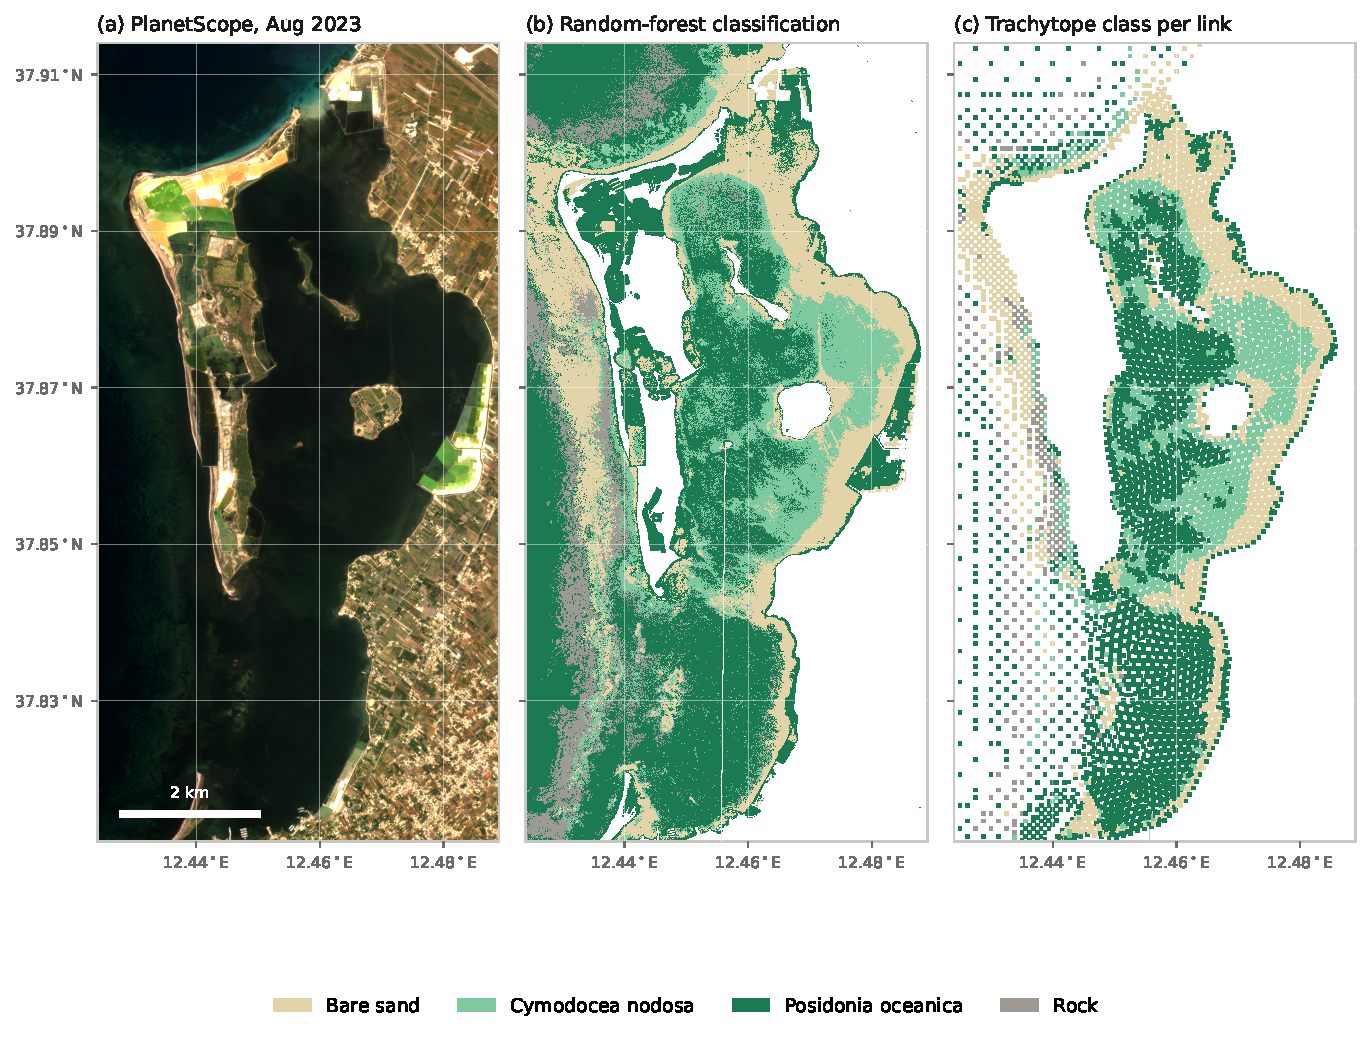
\includegraphics[width=\textwidth]{seagrass_classification}
  \caption{The seagrass map from imagery to model input. (a) PlanetScope
  SuperDove August 2023 median composite. (b) The random-forest classification,
  with the six output classes collapsed to the four seagrass classes.
  (c) The dominant class at each flow link, from the classification file
  the model reads, showing the mesh resolution the classification is sampled
  onto. The classification is computed over the whole scene, but only links
  inside the lagoon carry a canopy class.}
  \label{fig:seagrass}
\end{figure}

For reference, \citet{Ingrassia2024} obtained a best-fit uniform
Gauckler--Strickler coefficient of 20~m$^{1/3}$~s$^{-1}$ for the vegetated
Stagnone in a depth-averaged model, equivalent to a Manning coefficient of
0.050~s~m$^{-1/3}$.

\subsection{Observational data and validation metrics}
\label{sec:methods_validation}

Water level was recorded at ten-minute resolution at three stations, BocaNord
at the northern inlet, BocaSud near the southern inlet, and AltaVilaEst on the
eastern flank of the central basin. Offshore performance was assessed at the
Marettimo tide gauge.

Water-level skill was quantified with the raw root-mean-square error, the
bias, and the anomaly root-mean-square error computed after removing the
respective means, together with the linear correlation and the ratio of
modelled to observed standard deviation. The three error measures are related
by $\mathrm{RMSE}^2 = \mathrm{bias}^2 + \mathrm{RMSE}_{\mathrm{anom}}^2$, so
reporting them jointly separates a constant reference-level offset from
genuine dynamic error in phase and amplitude. The first simulated day was
discarded as spin-up, over which the initial condition relaxes and the
transients it generates leave the basin.

Lagrangian skill was assessed against GPS-tracked surface drifters released in
the lagoon interior during the simulation window. Simulated trajectories were
obtained by advecting particles with OpenDrift \citep{Dagestad2018} through the
modelled surface current field, at an advection step of 300~s and with
positions written every 600~s. Scoring was restricted, for each drifter, to
the interval between its first and last observation, since the advection
continues to the end of the forcing while the deployments last between 0.4 and
7.2~h. A wind drift factor of 0.02 was applied to every member. A sweep over
this parameter found no single value optimal across deployments, the optimum
instead falling as the mean wind speed rose, so a per-member or per-deployment
value would have confounded the process attribution with a tuning difference
and the one value was held fixed throughout.

Agreement was quantified with the normalised cumulative
Lagrangian separation skill score of \citet{Liu2011}, which accumulates the
separation between modelled and observed positions and normalises it by the
distance travelled by the observed drifter, and with the endpoint proximity,
the separation between modelled and observed positions at the end of each
deployment. \citet{Revelard2021} discuss the sensitivity of this class of
metric to the normalisation choice in coastal applications.

\subsection{Numerical experiments}
\label{sec:methods_experiments}

Eight simulations were run over the same nine-day window, from the same initial
condition and with identical boundary and atmospheric forcing, so that the
differences between them isolate individual model components. All eight share
the mesh, and all wrote station output every 600~s and gridded output every
1800~s, so the comparison is not affected by differences in output sampling.

Members are identified by a three-slot code whose slots mark wave coupling,
seagrass canopy and mobile bed in that order, carrying \texttt{W}, \texttt{V}
or \texttt{M} where the factor is active and a dash where it is not. The eight
are \texttt{{-}{-}{-}}, \texttt{{-}V{-}}, \texttt{W{-}{-}}, \texttt{WV{-}},
\texttt{{-}{-}M}, \texttt{{-}VM}, \texttt{W{-}M} and \texttt{WVM}, and the code
is used throughout the results.

The design is a complete factorial in three factors, wave coupling, seagrass
canopy and bed mobility, and all eight cells were obtained. Suspended sediment
does not contribute to the density field in the four mobile-bed members, which
therefore share that setting, and the fixed-bed members carry no sediment
module.

The setting is not a free parameter, since with suspended sediment feeding the
density field the two mobile-bed members without waves terminated on a
velocity overflow in a deep offshore cell, at the same cell and the same
simulated instant to six decimal places in the velocity. In a cell that deep
and carrying no erodible thickness, the baroclinic pressure gradient is the
only route by which advected sediment can move momentum, and restricting the
erodible layer by depth therefore leaves it untouched. Removing that
contribution completed both runs and also removed a spurious 2.4~m deposition
at 500~m depth, bringing the largest modelled bed-level change in the domain
inside the lagoon.

Erodible sediment is confined to depths at which waves can plausibly move it.
Available thickness is held at 0.5~m per fraction above 15~m depth and tapered
linearly to zero at 20~m, below which mean orbital velocity at the bed is
0.016~\si{\metre\per\second}, an order of magnitude below the range in which
the sand fraction mobilises. Without this restriction the bed erodes over the
whole domain, including water hundreds of metres deep where the process has no
physical meaning. The restriction bounds erosion and not deposition, so material
mobilised in shallow water still settles offshore.

The morphodynamic factor is a sensitivity test rather than a calibrated
prediction, the critical shear stress for erosion not having been constrained
against a repeated bathymetric survey.

The sensitivity to the numerical discretisation was tested outside the
factorial on the uncoupled fixed-bed configuration without canopy, under a
Courant limit of 0.5. Horizontal resolution was varied with a family of quadtree
meshes built in a conformal projection, with the domain, offshore grading and
open boundary of the present mesh, one bed surface common to the family and to
a run of the present mesh, and a cell edge of 60, 30 and 15~m inside the lagoon
and within 500~m of it. Vertical resolution was varied with
10, 20 and 40 uniform layers on the present mesh, run with the horizontal
momentum filter of the solver \citep{Deltares2025}, which the ensemble members
do not use. In the layer set the drifters were scored with the current of
the top layer and with the current averaged over the upper 0.04 and 0.2~m. The
uncoupled member was also repeated on four partitions on a second computer, to
test the dependence on the host and the decomposition.

